\documentclass[varwidth=true, border=5pt, convert={size=640x}]{standalone}
\usepackage{tikz}
\usetikzlibrary{positioning,shapes,arrows,backgrounds,calc,fit,trees,arrows.meta}
\newlength{\myimscale}
\renewcommand{\familydefault}{\sfdefault}
\begin{document}

\setlength{\myimscale}{0.05\textwidth}

\definecolor{kgrey}{HTML}{2b2828}

\begin{tikzpicture}[every node/.style={color=kgrey}]
\node[inner sep=0pt] (logo) at (3\myimscale,0\myimscale)
    {
\includegraphics[width=12\myimscale]{koopmans_grey_on_transparent.png}};
\node[rectangle, draw, thick, minimum width=5.75\myimscale, minimum height=3.5\myimscale, outer sep=0, label=above:linearisation,
           path picture={
               \node at (path picture bounding box.center){
                   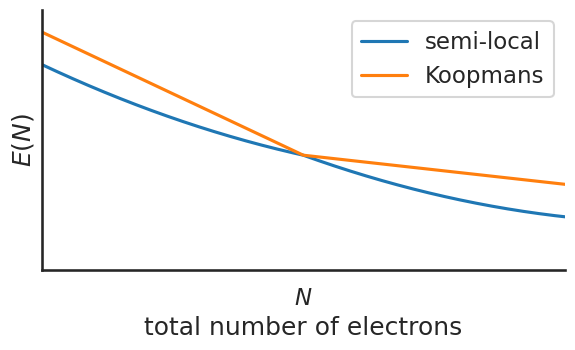
\includegraphics[width=5.75\myimscale]{linearisation.png}
               };
           }] (linear) at (0\myimscale,3.2\myimscale) {};
\node[rectangle, draw, thick, minimum width=5.75\myimscale, minimum height=3.5\myimscale, outer sep=0, label=above:screening,
           path picture={
               \node at (path picture bounding box.center){
                   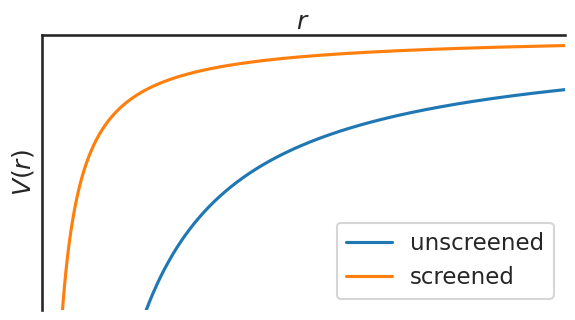
\includegraphics[width=5.75\myimscale]{screening.png}
               };
           }] (screening) at (6.25\myimscale,3.2\myimscale) {};
\node[rectangle, minimum width=2.5\myimscale, minimum height=3.5\myimscale, outer sep=0,
           path picture={
               \node at ([yshift=-0.05\myimscale]path picture bounding box.center){
                   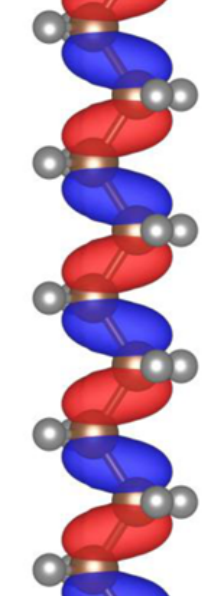
\includegraphics[width=2.5\myimscale]{fig_nguyen_canonical_orbital.png}
               };
           }] (bloch) at (-1.5\myimscale,-3.2\myimscale) {};
\node[rectangle, minimum width=2.5\myimscale, minimum height=3.5\myimscale, outer sep=0,
           path picture={
               \node at ([yshift=1.5\myimscale]path picture bounding box.center){
                   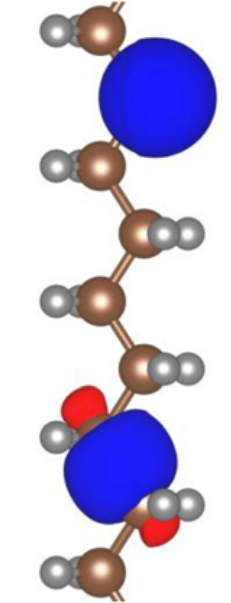
\includegraphics[width=2.6\myimscale]{fig_nguyen_variational_orbital.png}
               };
           }] (wannier) at (1.5\myimscale,-3.2\myimscale) {};
\node[rectangle, draw, thick, minimum width=5.75\myimscale, minimum height=3.5\myimscale, outer sep=0, label=below:localisation,
           ] (localisation) at (0\myimscale,-3.2\myimscale) {};
\node[rectangle, draw, thick, minimum width=5.75\myimscale, minimum height=3.5\myimscale, outer sep=0, label=below:automation,
           path picture={
               \node at (path picture bounding box.east){
                   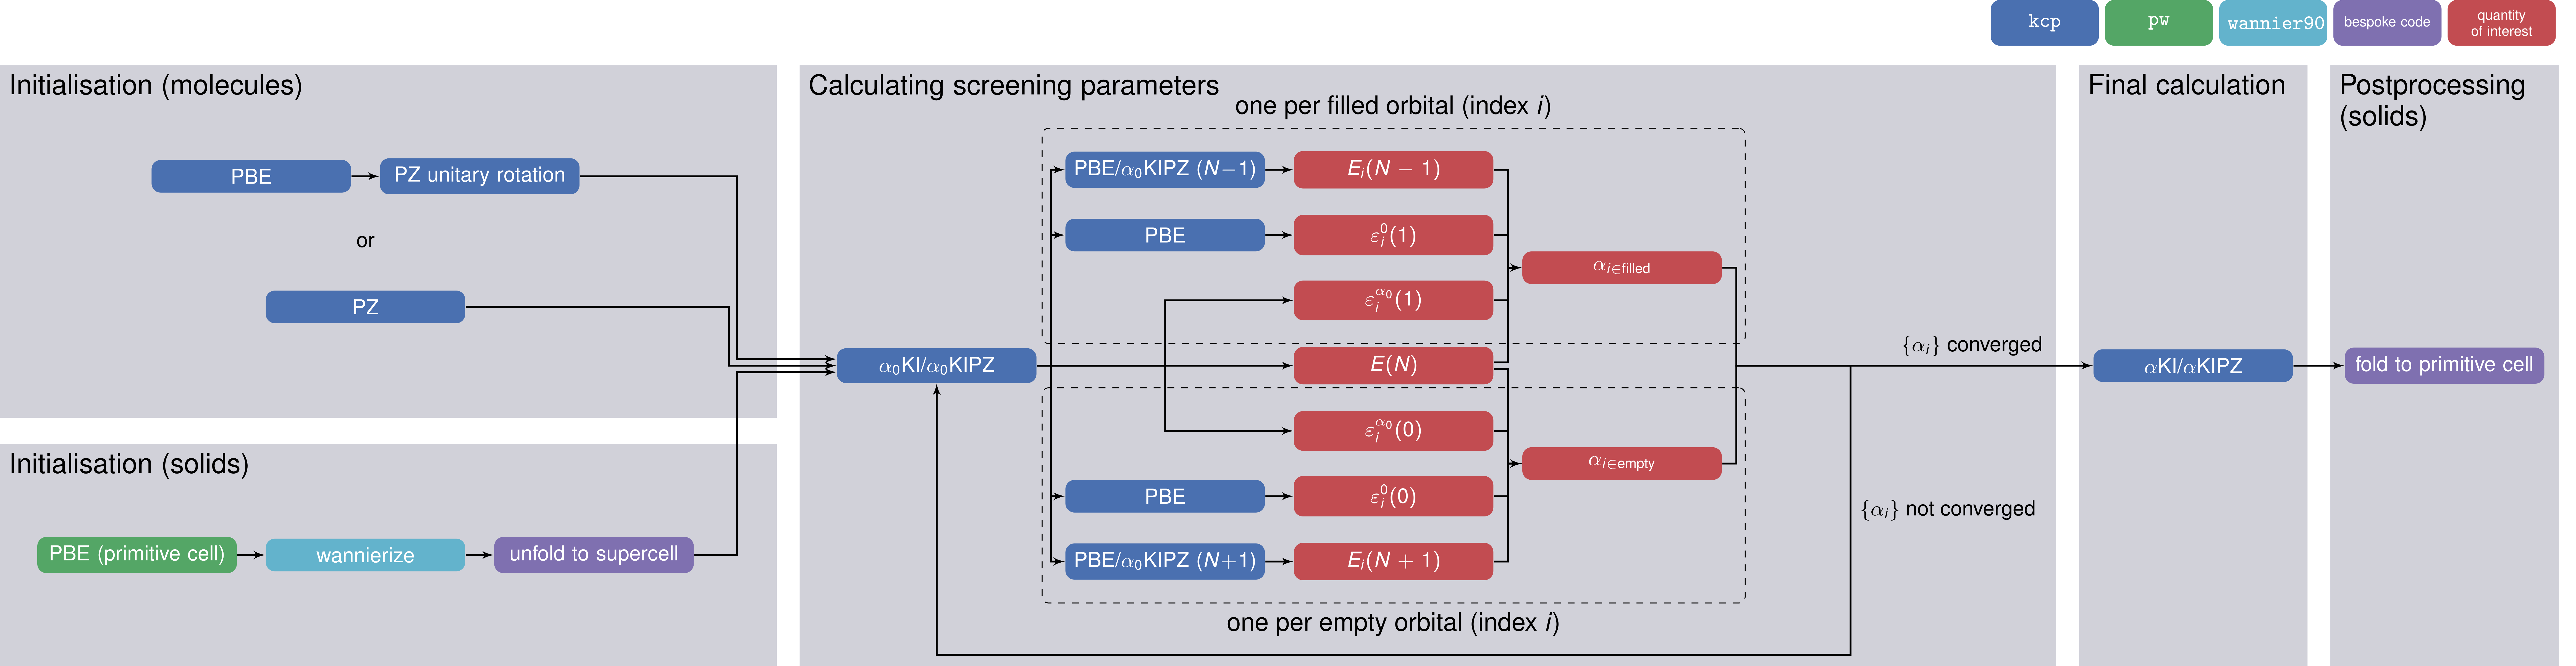
\includegraphics[width=15\myimscale]{dscf_workflow.png}
               };
           }] (workflow) at (6.25\myimscale,-3.2\myimscale) {};
\draw[thick, -{Latex[round]}] (bloch) -- (wannier);
\end{tikzpicture}
\end{document}
